\documentclass{ctexart}[UTF8]
\usepackage{dirtree}
\usepackage{listings}
\usepackage{xcolor}
\usepackage{graphicx}
\usepackage{enumerate}
\usepackage[a4paper]{geometry} 
\usepackage{amsmath,amsthm,mathtools,amssymb}
\usepackage{mathtools}
\usepackage{diagbox}
\usepackage{multirow,makecell}
\usepackage{float}
\usepackage{url}
\usepackage[nottoc]{tocbibind}
\usepackage{float}
\newcommand{\refe}[1]{Eq.\ref{#1}}
\newcommand{\reft}[1]{Theory.\ref{#1}\ }
\newcommand{\reff}[1]{图\ref{#1}\ }
\lstset{
 columns=fixed,
 numbers=left,                                        % 在左侧显示行号
 numberstyle=\tiny\color{gray},                       % 设定行号格式
 basicstyle=\small\ttfamily,
 frame=none,                                          % 不显示背景边框
 backgroundcolor=\color[RGB]{245,245,244},            % 设定背景颜色
 keywordstyle=\color[RGB]{40,40,255},                 % 设定关键字颜色
 numberstyle=\footnotesize\color{darkgray},           
 commentstyle=\color{gray}\ttfamily,                  % 设置代码注释的格式
 stringstyle=\rmfamily\slshape\color[RGB]{128,0,0},   % 设置字符串格式
 showstringspaces=false,
 breaklines=true,
 language=python
}
\newtheorem{theorem}{Theory}[section]
\geometry{bottom=2cm,left=1cm,right=1cm}
\title{上机9}
\author{张配天-2018202180}
\begin{document}
    \maketitle
    \tableofcontents
    \clearpage
    \section{问题描述}
    在滑完全程的前提下求最小的补水次数。
    \subsection{输入}
    补水点位置的数组$pos[n]$;
    \subsection{输出}
    最少的补水次数和补水位置;
    \section{算法思路}
    \subsection{最优子结构}
    假设最终最少的补水位置的序列为$\mathcal{H}^k = \{h_1,...,h_k\}$,$h_{*}$为补水站位置,其中有$h_i = pos[j]$,那么$\mathcal{H}^{i-1},\mathcal{H}^{i+1:k}$一定是
    最少补水位置序列;否则若存在更少的补水位置序列$\mathcal{H}^{i-1'}$,则由剪贴复制法,得到$\mathcal{H}^k$不是最少补水序列。
    \subsection{设计递归算法}
    在不补水就无法前往下一个补水点的时候补水,即若$(h_{i+1}-h_i)\cdot \frac{2}{m} > remain$,则在$h_i$补水。
    \subsection{证明贪心是安全的且最优解包含其中}
    \begin{theorem}
        设$\mathcal{H}_j \in \mathcal{H}^{j:k}$是第$j$次补水后的最少补水序列,$h_m$是第$j$次补水后最远能滑行到的补水地点,则$h_m$包含在$\mathcal{H}^{j:k}$中
    \end{theorem}
    \noindent\textbf{证明:}
    \begin{enumerate}
            \item 如果$\mathcal{H}_j[0] == h_m$,那么已经得证
            \item 否则,令$\mathcal{H}_j' = \mathcal{H}_j[1:] \cup h_m$,由于$h_m > \mathcal{H}_j[0]$,则替换$\mathcal{H}_j[0]$不会影响之后的补水序列$\mathcal{H}_{j+1}$,且总补水次数不变,因此$\mathcal{H}_j'$也是最优补水序列,得证。
        \end{enumerate}
    \section{复杂度分析}
    记补水站序列长度为$n$
    \begin{itemize}
        \item 第4-5行初始化,消耗时间$O(n)$
        \item 第12-17行便利补水站序列,按照上述规则挑选补水站进行补水,每次补水最多计算$O(1)$次,因此总时间复杂度$O(n)$
        \item 无需回溯,直接打印,复杂度$O(n)$
    \end{itemize}
    综上,整体算法时间复杂度$O(n)$,空间复杂度$O(n)$
    \section{源代码}
    \begin{lstlisting}
import numpy as np
total_length = 13
m = 2
pos = [0,1,2.6,4,4.2,4.4,5,6,7,8.1,9.2,9.5,10,11,12]
pos.append(total_length)

water_per_mile = 2/2

hydrate = []
remain = 2

for i,position in enumerate(pos[0:-1]):
    if (pos[i+1]-pos[i])*water_per_mile > remain:
        hydrate.append(position)
        remain = 2-(pos[i+1]-pos[i])*water_per_mile
    else:
        remain -= (pos[i+1]-pos[i])*water_per_mile

hydrate.append(total_length)
print(hydrate)
    \end{lstlisting}
    \section{运行截图}
    \begin{itemize}
        \item 自定义补水站序列为$[(0),1,2.6,4,4.2,4.4,5,6,7,8.1,9.2,9.5,10,11,12,(13)]$
        \item 自定义每公里耗水量为1公升
        \item 自定义线路总长度13公里
    \end{itemize}
    \begin{figure}[H]
        \centering
        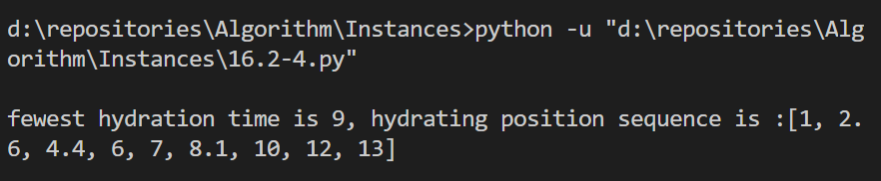
\includegraphics[width=14cm]{../Resources/9_1.png}
    \end{figure}
    经过验算,结果正确。
\end{document}